\documentclass[10pt, UKenglish]{beamer}
\usepackage{babel}
\usepackage[utf8]{inputenc}  
\usepackage{geometry}
\usepackage[customcolors]{hf-tikz}
\usepackage[T1]{fontenc}   
\usepackage{tcolorbox}
\usepackage{siunitx}
\usepackage{hyperref}
\usepackage{bookmark}
\usepackage{marvosym}
\usepackage{tikz}
\usepackage{tikz-qtree}
\usepackage{cancel}
\usepackage{todonotes}
\useoutertheme[subsection=false]{smoothbars}
\DeclareSIUnit[number-unit-product = {}]{\inchQ}{\textquotedbl}
\usepackage{amsmath,bm}
\DeclareSIUnit[number-unit-product = {\thinspace}]{\inch}{in}
\usetheme[menuwidth={0.3\paperwidth}]{erlangen}
\usepackage{multicol}
\usepackage{charter}
\setbeamercovered{transparent=20}
\setbeamertemplate{navigation symbols}{}
\sisetup{separate-uncertainty = true}
\usepackage[version=4]{mhchem}
\usepackage{tikz}
\usepackage{hepnames}
\usepackage{soul}
\usepackage{color}
\usepackage{thesis_defs}
\usepackage{subcaption}
\captionsetup[subfigure]{labelformat=empty}
\usepackage{xcolor}


\usepackage[backend=biber]{biblatex}
\bibliography{bibliography.bib}

\graphicspath{%
  {./feynman_diagrams/}%
  {./../../TRExFitter/NN_hadhad/Plots/}%
  {./figures_theory/}%
  {./figures_simple/}%
  {./figures_misc/}%
  {./app1/}%
  {./app2/}%
  {./app3/}%
}


\definecolor{color1}{RGB}{33,217,217}
\definecolor{color2}{RGB}{7,61,111}

\newcommand{\lr}{\mathcal{lr}}


\newcounter{totavalue}
\newcounter{parvalue}

\def\aux{1}
\def\radius{9pt}
\def\step{4pt}
\usepackage[absolute,overlay]{textpos}


\newcommand\circcounter{%
\ifnum\inserttotalframenumber<2\relax
\else
  \setcounter{totavalue}{\inserttotalframenumber}
  \setcounter{parvalue}{\insertframenumber}
  \ifnum\inserttotalframenumber>45\relax
    \renewcommand\step{0pt}
  \fi%
  \pgfmathsetmacro{\aux}{360/5}
  \begin{tikzpicture}[remember picture,overlay, rotate=90+\aux]
  \foreach \i in {0,1,...,5}
    \fill[logo_blue] 
      (0,0) -- (-\i*\aux:\radius) arc  (-\i*\aux:-(\i+1)*\aux+\step:\radius) -- cycle;
  \foreach \i in {1,...,\insertframenumber}
    \fill[logo_grey] 
      (0,0) -- (-\i*\aux:\radius) arc  (-\i*\aux:-(\i+1)*\aux+\step:\radius) -- cycle;
  \fill[white] circle (\radius/1.3);
  \node at (0,0) {\small\insertframenumber}; 
  \end{tikzpicture}%
\fi%
}


\usepackage{eso-pic,picture}



\begin{document} 

\title[Bachelorvortrag]{Meetings - A workshop summary}
\subtitle{22nd of April}
\author{Christian Kirfel}
%\institute{Universtität Bonn}
        



\begin{frame}[plain]
\vspace{0.0cm}
  \titlepage
      \AddToShipoutPictureFG*{%
    \AtPageUpperLeft{%
      \put(8.7cm,-9.6cm){

\includegraphics[scale=0.03]{original_logo.jpg}
\makebox(0,0)[lt]{}%
      }%
    }%
  }%
    \AddToShipoutPictureFG*{%
    \AtPageUpperLeft{%
      \put(0.0cm,-9.6cm){
%\includegraphics[scale=0.17]{atlas_gay.png}
%
\includegraphics[scale=0.17]{ATLAS-Logo-Ref-RGB-H_0.jpg}
\makebox(0,0)[lt]{}%
      }%
    }%
  }%
\end{frame}
\addtobeamertemplate{navigation symbols}{\vspace*{0.8cm}\hfill\circcounter\hspace*{0.7cm}}


%\section{Teaching}
%\begin{frame}{Teaching}
\begin{itemize}
\item Done! :)
\end{itemize}
\end{frame}
%\section{QT}
%\begin{frame}{QT updates}
\begin{itemize}
\item Created several comparison presenations last week
\item Improved plot qulatiy, now using the up to date comparison script
\item Updated tutorial and moved it to a repo (now with the rare feature of actually working)
\end{itemize}
\end{frame}
%\section{Analysis}
%\begin{frame}{Motivation}
	\begin{itemize}
		\item Speed up the tedious process of hyperparameter optimisation
		\item Overcome the issue of optimal architecture being highly problem dependent
		\item Avoid biased decision of an expert user
		\item Utilize the baf job submission structure to efficiently run large samples of small optimisation jobs
	\end{itemize}
\end{frame}

\begin{frame}{Theory}
	\begin{itemize}
		\item Code inspired by \cite{naranjo}
		\item Use a $(\lambda + \mu)$ scheme.
		\item $\lambda$ individuals per generation
		\item $\mu$ individuals selected to create the next generation
	\end{itemize}
	\begin{figure}
    	\centering
		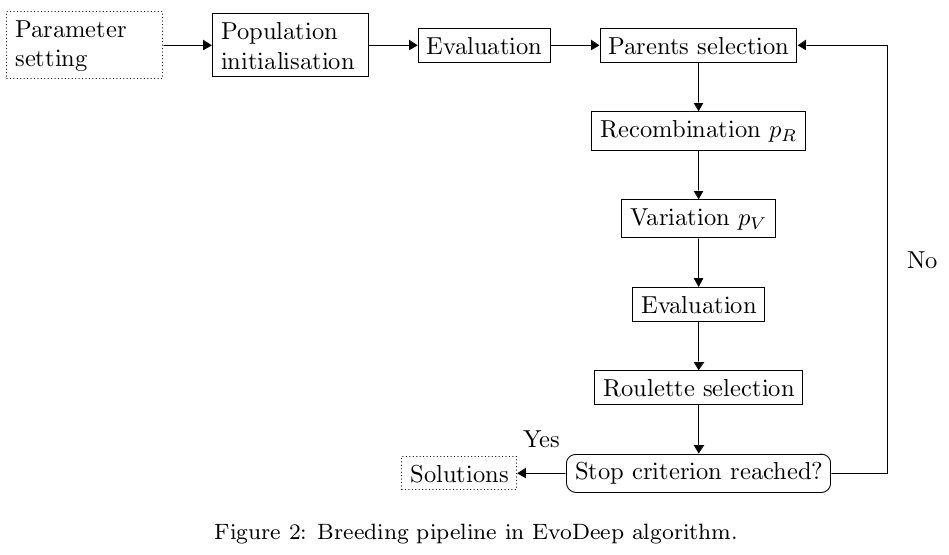
\includegraphics[width=0.8\textwidth]{breed.png}
    \end{figure}
\end{frame}

\begin{frame}{Baf setup}
	\begin{enumerate}
		\item A bash script submits a badge of jobs from the local machine
		\item The script waits for all jobs to finish
		\item The jobs are evaluated based on AUC and Accuracy
		\item Based on the evaluation, a new set of jobs is created
		\item Remnants of the old submission are removed to avoid exceeding quota
	\end{enumerate}
\end{frame}

\begin{frame}{Early results}
	\begin{itemize}
		\item Testing tZ versus ttbar
		\item Tested for Lorentz-Invariant and basic kinematic variables
		\item Testing on nodes, layers, learning rate, dropout
		\item The network ends around:
		\item Testing for similarity of final paramters. Even for small test samples the parameters are very similar
		\item Plots soon to come, unfortunately I had some plotting issues that are now fixed
	\end{itemize}
\end{frame}

\begin{frame}{Conclusion and future steps}
	\begin{itemize}
		\item Running smoothly on baf for all test runs
		\item The network is approaching a reasonable order of magnitude and getting closer every single step
		\item Unreasonable genotypes are discarded
		\item Biggest impact made by epochs and metrics
		\item Weight ini has to be checked
		\item Starting parameters have to bet set. Lately some runs resulted in bad parameters
	\end{itemize}
\end{frame}



\begin{frame}
  \begin{center}
  \Huge Pünktlichkeit ist die Höflichkeit der Könige.
  %Why do I mention this. Well. Often times we poison our relationships and meeting atmosphere by accepting unnecessary behaviour.
  %Behaviour we despise but feel like it is impolite to speak up about
  \end{center}
\end{frame}

\begin{frame}{Tips for efficient meetings}
  \begin{itemize}
    \item Define the objectives of the meeting. Otherwise, no decision will be made.
    \item Create and agenda and stick to it. Make sure people only talk about one topic at a time.
    \item Keep the circle of participants small. If decisions are to be made, invite no more than 6 people.
    \item Invite only people who are essential. Avoid making the meeting a ritual.
    \item Keep it short, not more than 45 minutes.
  \end{itemize}
\end{frame}


\begin{frame}{Tips for efficient meetings}
  \begin{itemize}
    \item Make sure the mood is positive.
    \item Conduct the meeting in a strict but collegial manner.
    \item Separate person and subject.
    \item Never criticise in front of others.
    \item Let the leadership rotate among the participants.
    \item Give an employee the opportunity to leave when the agenda topics than concern him have been covered.
  \end{itemize}
\end{frame}

\begin{frame}{Tips for efficient meetings}
  \begin{itemize}
    \item Distinguish between informative meetings and decision-making meetings.
    \item Stop denying the limitation of attention spans.
    \item Admit to yourself if a meeting annoys you, improve your own efficiency.
    \item Agenda, timeslots, punctuality are important elements to keep a positive atmosphere.
  \end{itemize}
\end{frame}

%\begin{frame}{Forward jet}
    \begin{columns}
        \begin{column}{0.5\textwidth}
            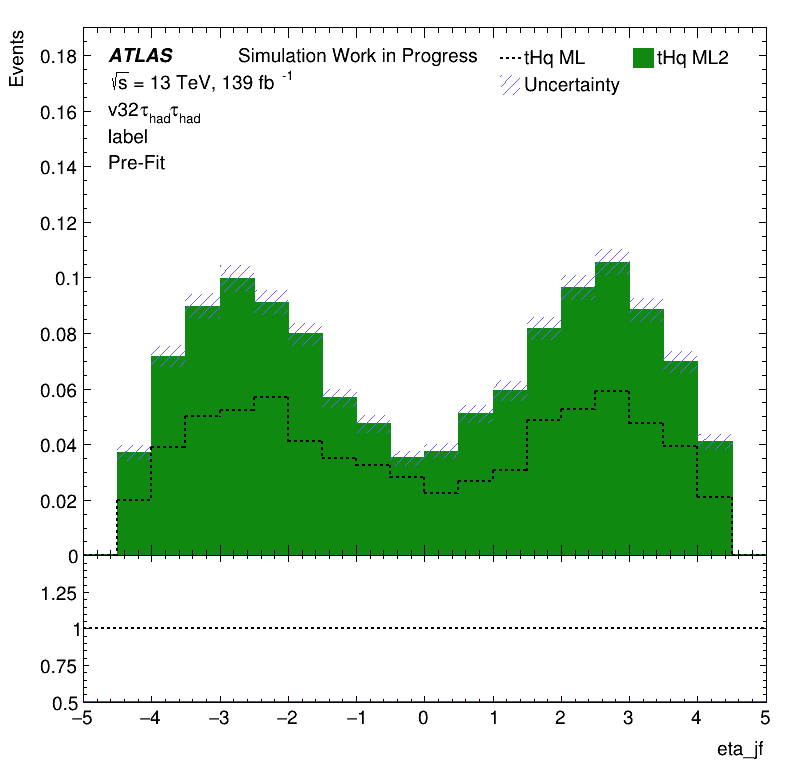
\includegraphics[width=0.75\textwidth]{eta_jf.png}
        \end{column}
        \begin{column}{0.5\textwidth}
            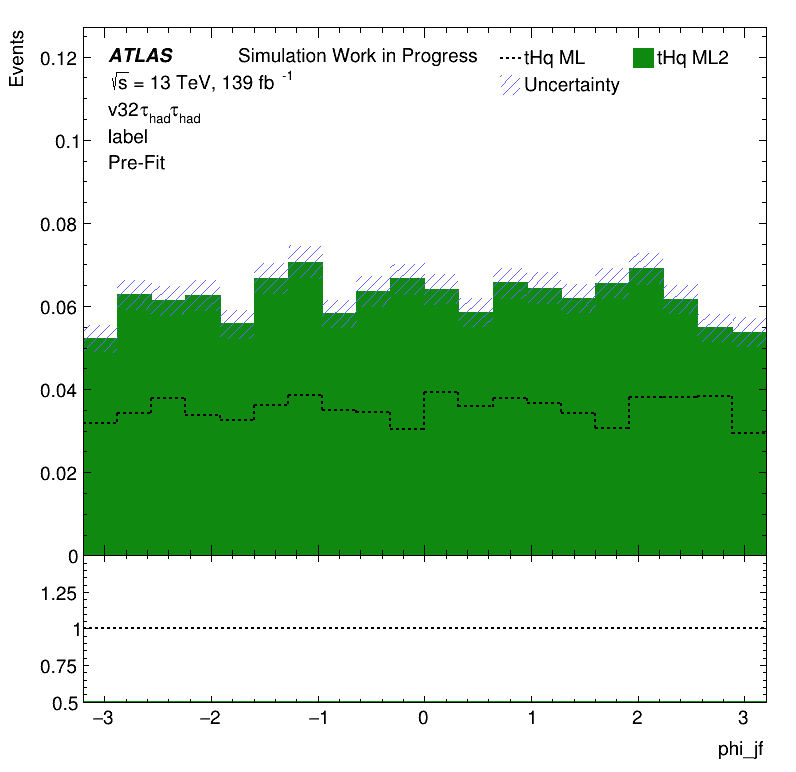
\includegraphics[width=0.75\textwidth]{phi_jf}
        \end{column}
    \end{columns}
            \centering 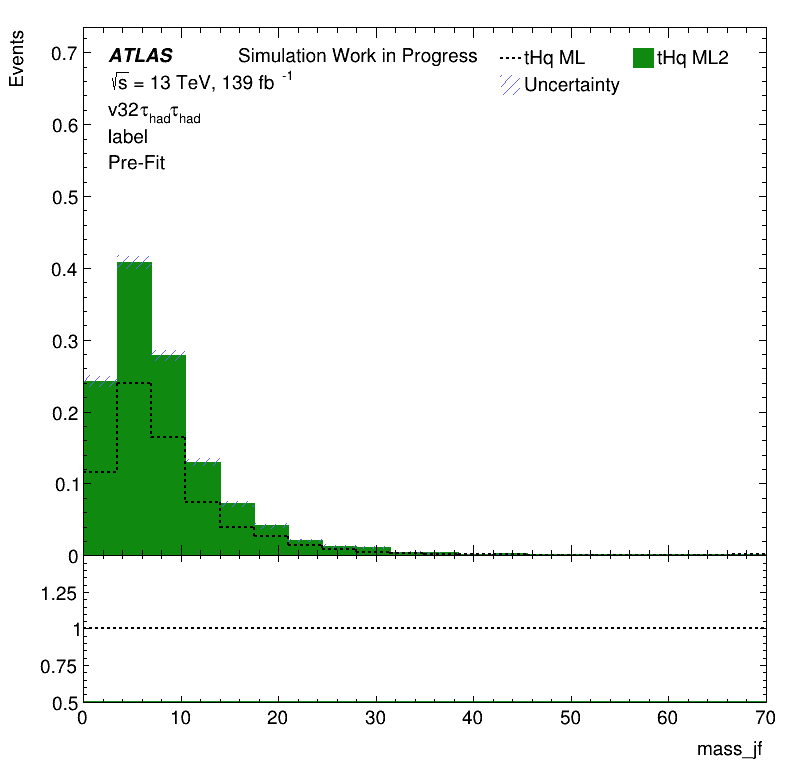
\includegraphics[width=0.37\textwidth]{mass_jf}
\end{frame}

\begin{frame}{B jet}
    \begin{columns}
        \begin{column}{0.5\textwidth}
            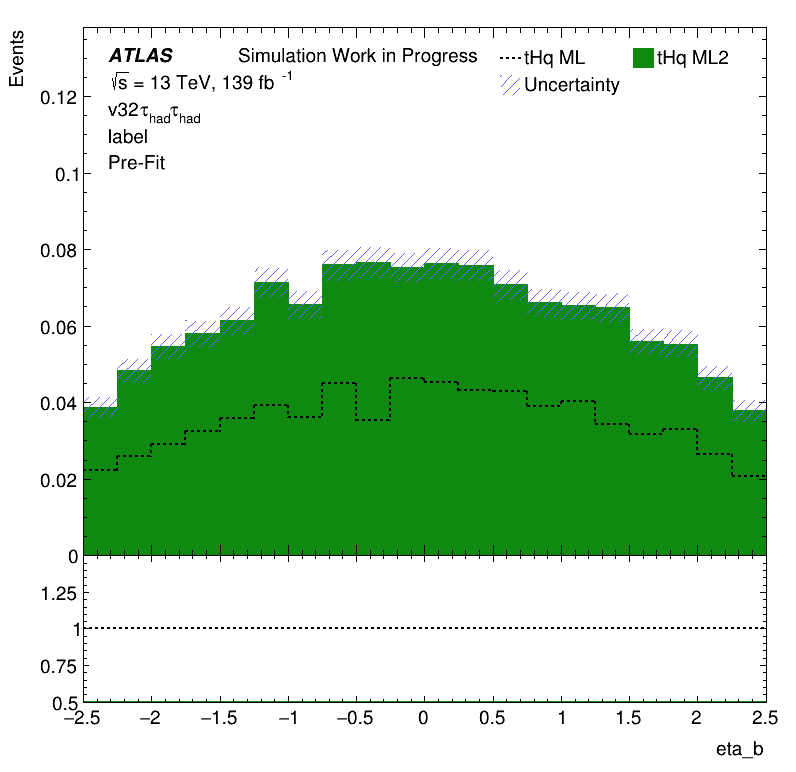
\includegraphics[width=0.75\textwidth]{eta_b.png}
        \end{column}
        \begin{column}{0.5\textwidth}
            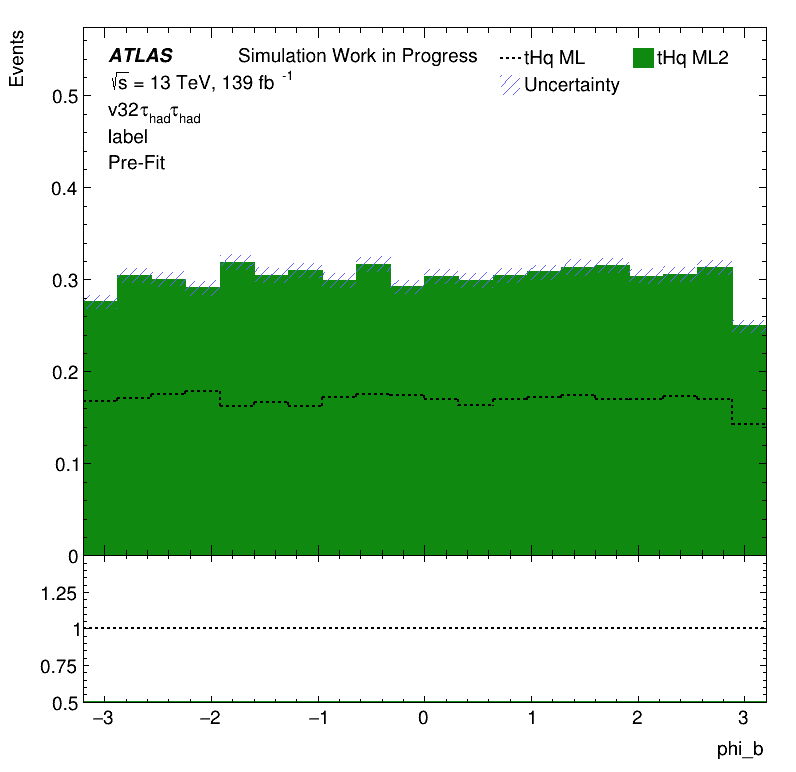
\includegraphics[width=0.75\textwidth]{phi_b}
        \end{column}
    \end{columns}
            \centering 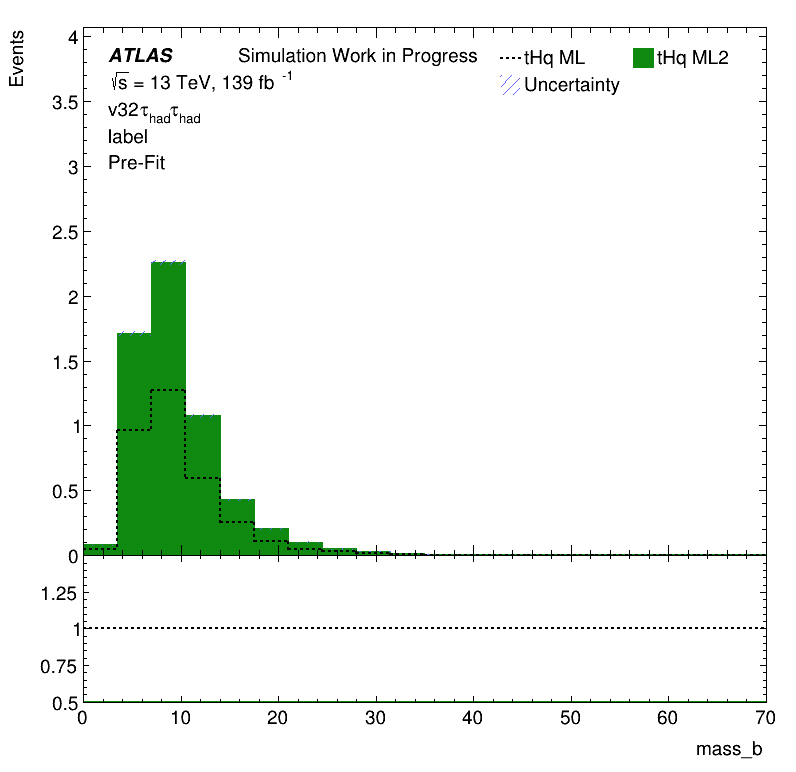
\includegraphics[width=0.37\textwidth]{mass_b}
\end{frame}

\begin{frame}{Reconstructed Higgs}
    \begin{columns}
        \begin{column}{0.5\textwidth}
            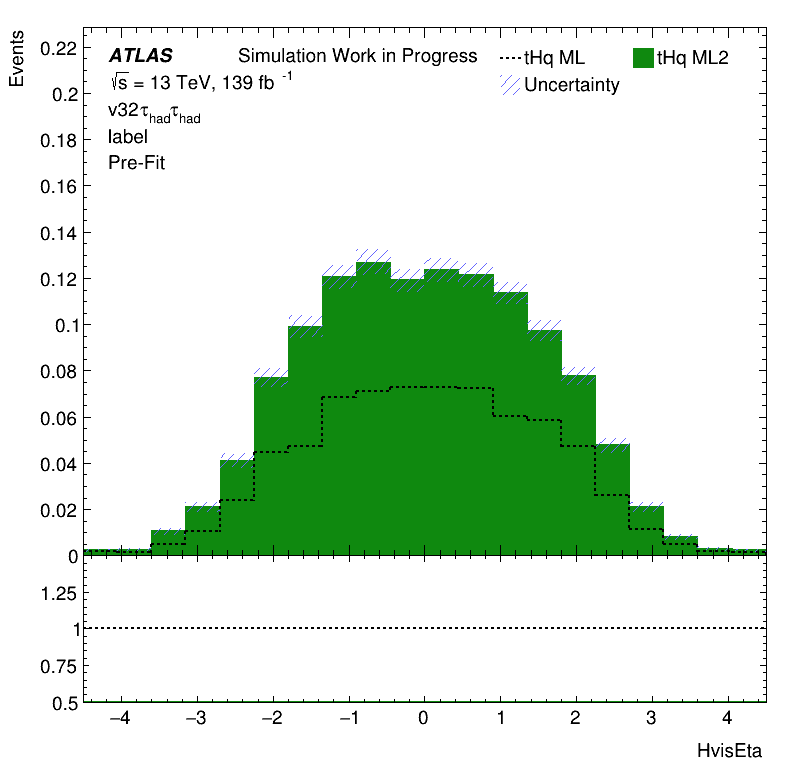
\includegraphics[width=0.75\textwidth]{HvisEta.png}
        \end{column}
        \begin{column}{0.5\textwidth}
            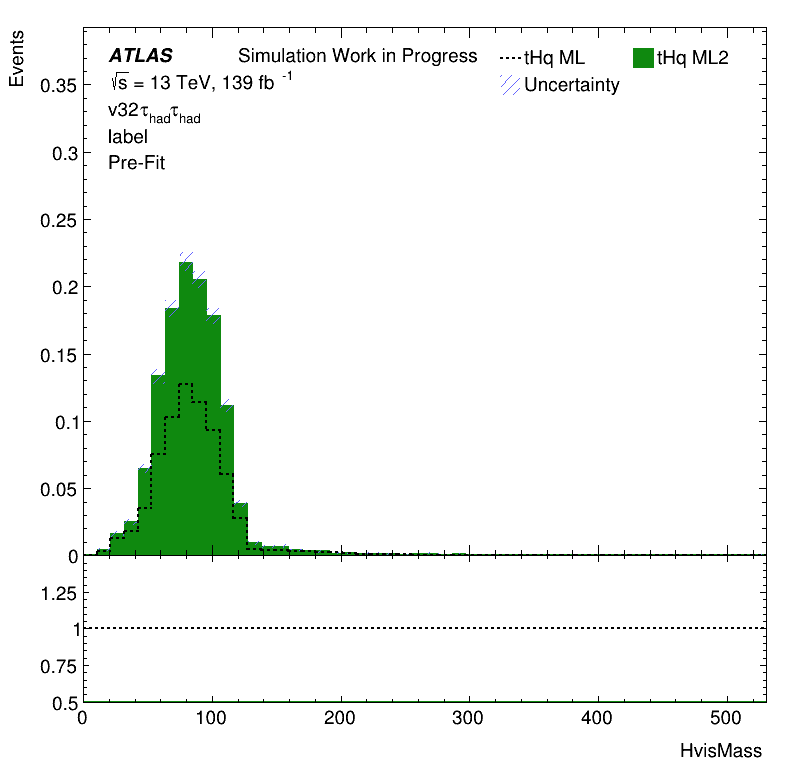
\includegraphics[width=0.75\textwidth]{HvisMass}
        \end{column}
    \end{columns}
            \centering 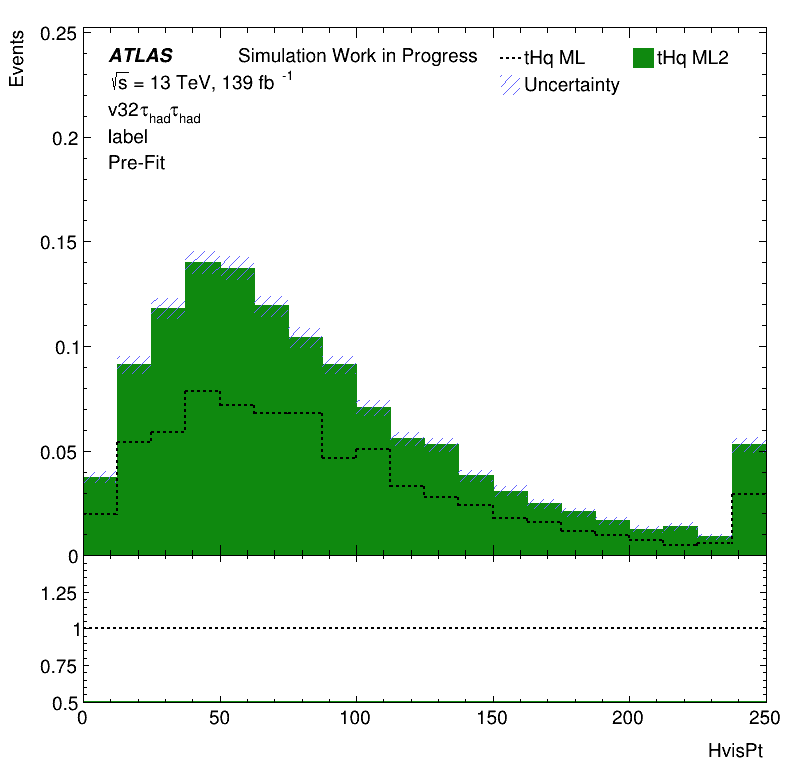
\includegraphics[width=0.37\textwidth]{HvisPt}
\end{frame}

\begin{frame}{Reconstructed Top}
    \begin{columns}
        \begin{column}{0.5\textwidth}
            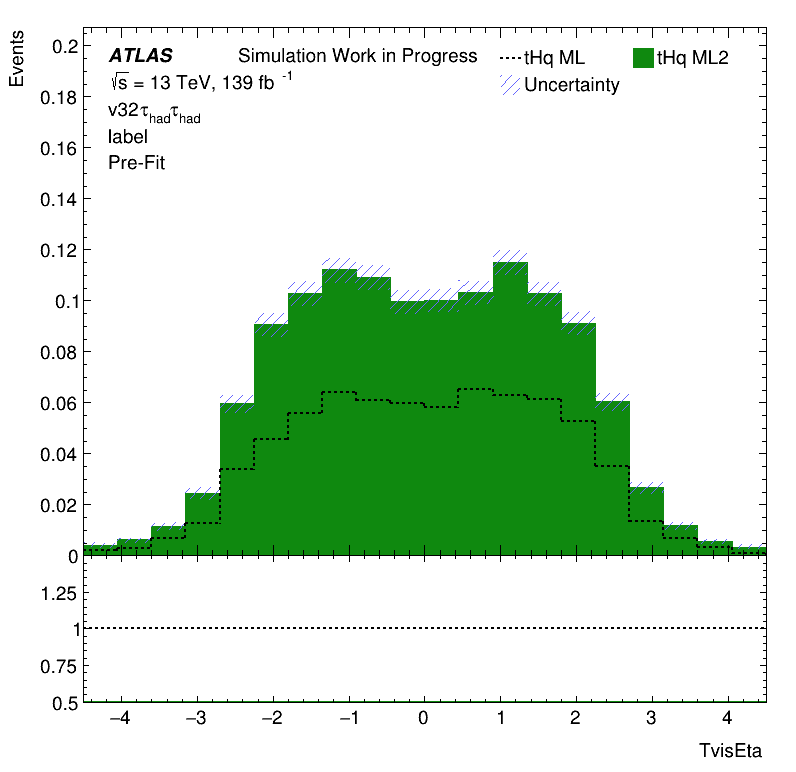
\includegraphics[width=0.75\textwidth]{TvisEta.png}
        \end{column}
        \begin{column}{0.5\textwidth}
            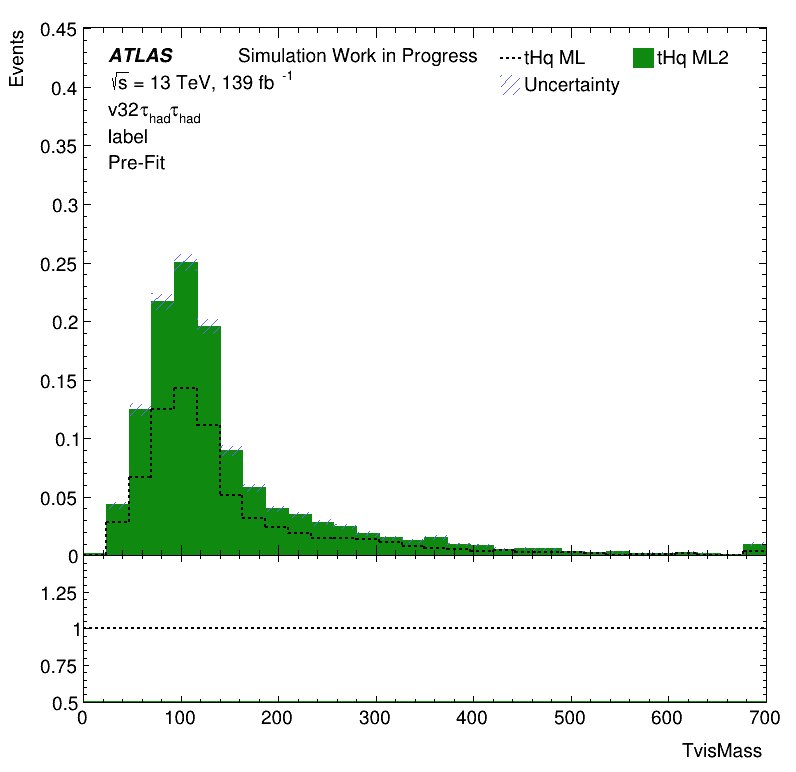
\includegraphics[width=0.75\textwidth]{TvisMass}
        \end{column}
    \end{columns}
            \centering 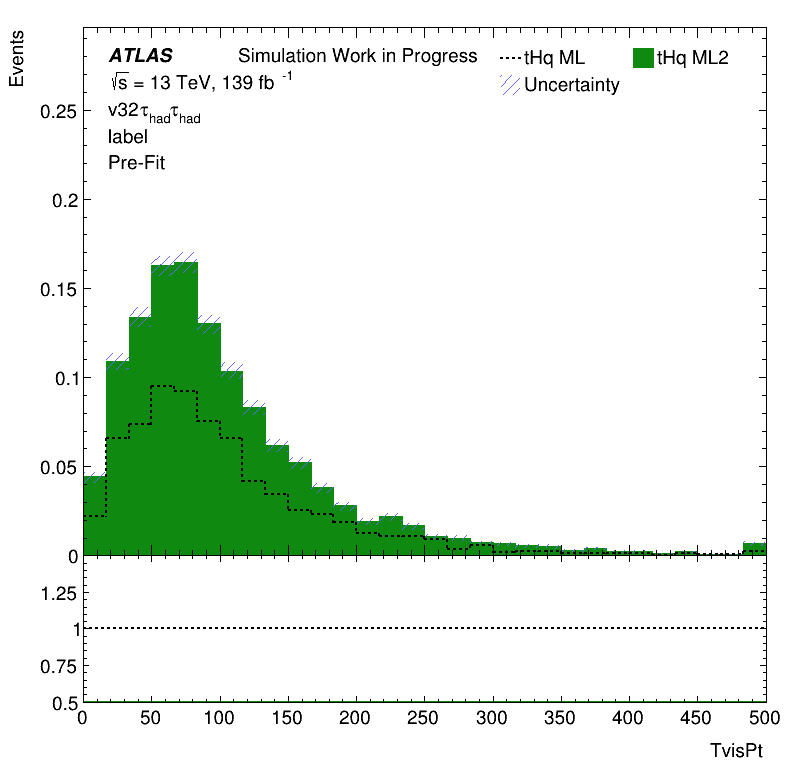
\includegraphics[width=0.37\textwidth]{TvisPt}
\end{frame}

%\begin{frame}{Sources}

%\printbibliography
    
%\end{frame}






\end{document}